\documentclass{beamer}
\usepackage[spanish]{babel}
\usepackage[utf8]{inputenc}
\usepackage {graphicx}
\title[Distribución Geométrica]{Estudio de la función de Distribución Geométrica}
% AUTOR (\fntx es un tipo de fuente definida en el paquete de estilo)
\author[M.Baeza,J.J.Dóniz,J.Rdguez]{
        María Baeza López\\
        Juan Jesús Dóniz Labrador \\
        Jesús Rodríguez Falcón\\
      }

\institute{Matemáticas}
\date[15/05/2014  ULL]{La Laguna,15 de Mayo de 2014}
\usetheme{Madrid}
\definecolor{MiVioleta}{RGB}{122,59,122}
\definecolor{MiAzul}{RGB}{0,88,147}
\definecolor{MiGris}{RGB}{56,61,66}
\setbeamercolor*{palette primary}{use=structure,fg=white,bg=MiVioleta}
\setbeamercolor*{palette secundary}{use=structure,fg=white,bg=MiAzul}
\setbeamercolor*{palette tertiary}{use=structure,fg=white,bg=MiGris}
\begin{document}
\begin{frame}

\includegraphics[width=0.15\textwidth]{img/ullesc.jpg}
  \hspace*{3cm}
  
\includegraphics[width=0.16\textwidth]{img/fmatesc.jpg}
  \hspace*{3cm}
  
\includegraphics[width=0.16\textwidth]{img/ullesc.jpg}
\titlepage
\end {frame}
\begin{frame}
\frametitle{Indice}
\tableofcontents[pausesections]
\end {frame}
\section {Introducción}
\begin{frame}
\frametitle{Introducción}
En este trabajo hemos elaborado un función Python que resuelva problemas matemáticos asociados a la función de distribución geométrica. \\

Para ello hemos recopilado información sobre dicha función,también hemos probado y verificado que la función que se ha implementado funciona correctamente,además de comprobar la eficacia de la misma.
\end {frame}
\section {Fundamentos Teóricos}
\begin{frame}
\frametitle{Distribución Geométrica}
La distribución geométrica es un modelo adecuado para aquellos procesos en los que se repiten pruebas consecutivamente hasta obtener el resultado correcto o deseado (éxito).
Esta distribución se puede expresar de las siguientes maneras:
\begin{itemize}
\item[$\rightarrow$]La distribución de probabilidad del número X necesaria para obtener un éxito, contenido en el conjunto $\lbrace 1,2,3,... \rbrace$ \pause
\item[$\rightarrow$]La distribución del número $Y=X-1$ de fallos antes del primer éxito,contenido en el conjunto $\lbrace 1,2,3,... \rbrace$
\end{itemize}
\end{frame}
\begin{frame}
\frametitle{Función de Probabilidad}
La función de probabilidad de esta distribución se puede escribir de dos maneras posibles, dependiendo la definición de la función de distribución:
\begin{itemize}
\item[$\rightarrow$]Si la probabilidad de éxito en cada caso es p, entonces la probabilidad de que x ensayos sean necesarios para obtener un éxito es: \pause
\begin{block}{}
\[P(X=x)=(1-p)^{x-1} \cdot p \;\; \textsf{, para} \;\; x=0,1,2,3,...\]
\end{block} \pause
\item[$\rightarrow$]Equivalentemente, la probabilidad de que haya x fallos antes del primer éxito es: \pause
\begin{block}{}
\[P(X=x)=(1-p)^{x} \cdot p \;\; \textsf{, para} \;\; x=0,1,2,3,...\]
\end{block}
\end{itemize}
\end{frame}
\begin{frame}
\frametitle{Propiedades de la función Geométrica}
\begin{itemize}
\item[$\rightarrow$]La media:
\[ E(X) = \frac{1}{p} \;\;\;\; \textsf{o} \;\;\;\; E(Y) = \frac{1-p}{p}\] \pause
\item[$\rightarrow$]La varianza:
\[ V(X) = V(Y) = \frac{1-p}{p^2}\] \pause
\item[$\rightarrow$]La moda:es el valor de la variable que tiene asociada la mayor probabilidad. Es fácil ver que:
\[P(x_i) \leq P(X=1) \;\forall x_i \] \pause
\item[$\rightarrow$]La mediana se define como:
\[Me = \frac{-ln(2)}{ln(q)}\]
\end{itemize}
\end{frame}
\section {Procedimiento experimental}
\begin{frame}
\frametitle{Funciones utilizadas en Python}
% Iria el Código de las dos funciones
En primer lugar implementamos dos funciones que resolvieran los diversos problemas relacionados con la distribución geométrica:
\begin{center}
\hyperlink{Liga1}{\beamergotobutton{Código de funciones}}
\hypertarget<2>{Liga2}{}
\end{center}

Después de comprobar que ambas funcionaban correctamente, comenzamos a implementar el código principal que cubría todos los casos posibles, quedando como sigue:
\begin{center}
\hyperlink{Liga3}{\beamergotobutton{Código principal}}
\hypertarget<2>{Liga4}{}
\end{center}
\end{frame}
\begin{frame}
\frametitle{Ejemplo}
\begin{block}{\color{white}Problema 2: Tantos en baloncesto}
Un jugador de baloncesto no cesa en su intento de lanzar pelotas a la canasta que se halla situada a 2 metros de altura hasta que consiga introducir una de éstas a través del aro. Si se supone que sus tiros son independientes y que la probabilidad de anotar una canasta es de 0.8,¿ cuál es la probabilidad de que el baloncestista necesite realizar dos tiros?¿ y de que sean tres tiros, cuatro tiros, cinco tiros, etc. hasta deducir la fórmula para n tiros?¿ cuál es la probabilidad de necesitar como mucho cinco tiros?
\end{block}

\leftline{\Large{\bf Solución:}}

Supongamos que tenemos la siguiente variable aleatoria:
\begin{center}
\bf{X = número de tiros necesarios por el baloncestista hasta anotar una canasta}
\end{center}
Ahora bien, sabemos que los valores de p y q son los siguientes:
\begin{center}
{$p=0.8;\; q=1-p= 1-0.8= 0.2$}
\end{center}
\end{frame}
\begin{frame}
\frametitle{Ejemplo}
Procedamos por tanto, a calcular dichas probabilidades:
\begin{itemize}
\item [$\rightarrow$]{$P[X=1]=  p= 0.8 $} \pause
\item [$\rightarrow$]{$P[X=2]= q\cdot p= 0.8\cdot 0.2 = 0.16$} \pause
\item [$\rightarrow$]{$P[X=3]= q\cdot q\cdot p= 0.8\cdot 0.8\cdot 0.2 = 0.032$} \pause
\item [$\rightarrow$]{$P[X=4]= q\cdot q\cdot q\cdot p= 0.8\cdot 0.8\cdot 0.8\cdot 0.2 = 0.0064$} \pause
\item [$\rightarrow$]{$P[X=5]= q\cdot q\cdot q\cdot q\cdot p= 0.8\cdot 0.8\cdot 0.8\cdot 0.8\cdot 0.2 = 0.00128$}
\end{itemize}
Luego, de aquí es fácil apreciar que:
\begin{block}{Fórmula}
{\[P[X=n]= q^{n-1}\cdot p\]}
\end{block} \pause
Veamos ahora cuál es la probabilidad de necesitar como máximo cinco tiros para encestar en la canasta. Atendiendo a los resultados del apartado anterior nos queda:
\begin{center}
{$P[X\leq5]=0.8 + 0.16 + 0.032 + 0.0064 +0.00128 = 0.99968$}
\end{center}
\end{frame}
\begin{frame}
\frametitle{Ejemplo}
En Python se calcularía:
\begin{itemize}
  \item[$\rightarrow$]En primer lugar meteríamos en Konsole la sentencia: \textbf{python geo\_ sol.py n 0.8}, donde n va variando entre 1 hasta 5
  \item[$\rightarrow$]Seguidamente el programa te manda a elegir una opción de las ofertadas: para las cinco primeras veces escogeremos la \textbf{opción 0} y para la última la \textbf{opcion 1}:
  \begin{itemize}
  	\item[$\circ$]La \textbf{opción 0} es la más sencilla y solo utiliza la función: \textbf{def calcular\_ geo (n,p)}
  	\item[$\circ$]La \textbf{opcion 1} necesita de las dos funciones implementadas: la anterior llamada dentro de la función \textbf{def calcular\_ geo1 (n,p)}
  \end{itemize}
  \item[$\rightarrow$]Por último, el programa te dará los resultados y el tiempo que ha tardado en calcularlo.
\end{itemize}
\end{frame}
\begin{frame}
\frametitle{Resultados obtenidos}
En la siguiente tabla se muestran los resultados obtenidos durante la comprobación de la función:
\begin{center}
\scalebox{0.55}{
\begin{tabular}{|c||l||l||p{2.5cm}||p{2.5cm}||p{2.5cm}||p{2.5cm}||}
\hline
\textbf{Problemas:  } & \textbf{p} &\textbf{Resultado Python (1) }& \textbf{Resultado ''a mano''(2)} & \textbf{Calculadora Online}(3) & \textbf{Error entre (1) y (2)} &  \textbf{Error entre (1) y (3)} \\ \hline
 1 & 0.5 & $P[X\geq 2]=0.25$ & $\frac{1}{4}$ & 0.25 & 0 & 0   \\
 2 & 0.8 & $P[X=1]=0.8$ & 0.8 & 0.8 & 0 & 0 \\
   & 0.8 &$P[X=2]=0.16$ & 0.16 & 0.16 & 0 & 0\\
   & 0.8 &$P[X=3]=0.032$ & 0.032 & 0.0032 & 0 & 0 \\
   & 0.8 &$P[X=4]=0.0064$ & 0.0064 & 0.0064 & 0 & 0\\
   & 0.8 &$P[X=5]=0.001280$ & 0.0013 & 0.00128 & $2\cdot 10^{-6}$ & 0 \\
   & 0.8 &$P[X\leq 0]=0.999680$ & 0.99968 & 0.99968 & 0 & 0\\
 3 & 0.16666666 &$P[X=3]=0.115741$ & 0.1157 &  0.115773796296 & $4.1\cdot 10^{-5}$ & $3.04\cdot 10^{-6}$ \\
 4 & 0.4 &$P[X<3]=0.64$ & 0.64 & 0.64 & 0 & 0 \\
 \hline

\end{tabular}
}
\end{center}
Como se puede observar los errores que se producen son nulos o cantidades mínimas, debido sobre todo a las aproximaciones de los valores p introducidos al programa.
\end{frame}
\begin{frame}
\frametitle{Tiempos obtenidos}
En la siguiente gráfica podemos observar los tiempos (en segundos) obtenidos al hacer los cálculos con el valor $p=0.3$:
\begin{figure}[H]
\begin{center}
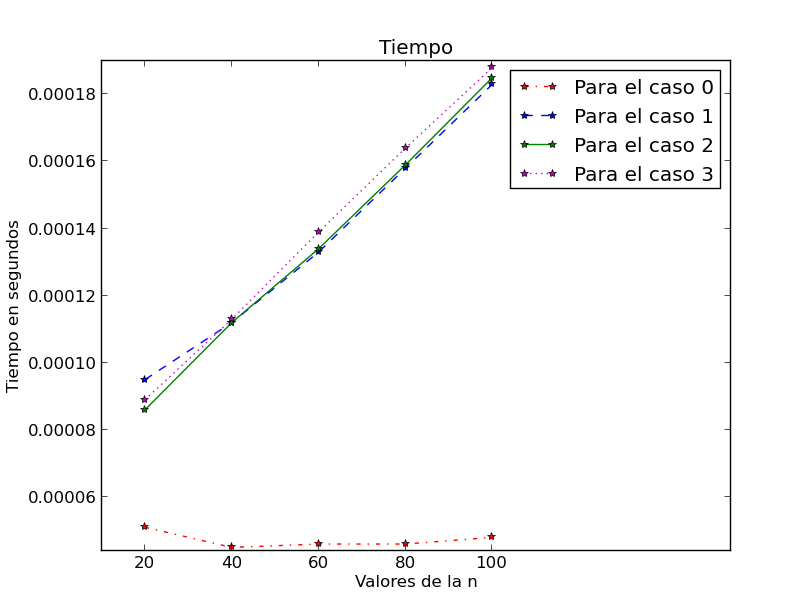
\includegraphics[width=0.65\textwidth]{img/figura1.png}
\caption{Gráfica de resultados}
\label{fig:1}
\end{center}
\end{figure}
\end{frame}
\section {Conclusiones}
\begin{frame}
\frametitle{Conclusiones}
Podemos sacar como conclusión final que:
\begin{enumerate}
  \item Debemos ejecutar varias veces un programa, hasta purificarlo y sacar un programa eficiente y operativo. \pause
  \item Además, gracias a nuestra búsqueda de información hemos podido refrescar y ampliar conocimientos sobre probabilidades, más concretamente sobre la distribución geométrica. \pause
   \item Nos hemos dado cuenta del enorme potencial que tiene la utilización de \LaTeX, Beamer y Python, para la elaboración documental, de presentación y de creación de algoritmos, respectivamente. Nos será de gran ayuda en la elaboración de nuestros escritos, en el marco de nuestra formación académica universitaria y laboral.
\end{enumerate}
\end{frame}
\begin{frame}
\frametitle{Bibliografía}
\begin{thebibliography} % Esta inventada es de la practica 11
\beamertermplatebookbibitems
\bibitem[Ejercicios resuestos de probabilidad,2001]{pro1}
Ejercicios resueltos de probabilidad (Año 2001)
{\small Salazar Gonz\'alez JJ y L\'opez Yurda M}
\bibitem[Estadistica I.Probabilidad y distribuciones,2000]{pro2}
Estadistica I.Probabilidad y distribuciones (Año 2000)
{\small Casas  S\'anchez JM y Zamora  Sanz A}
\bibitem[Calculadora de la distribución geométrica(2011)]{URL}
 Calculadora de la distribución geométrica (2011)
{\small $http://www.elektro-energetika.cz/calculations/distrgeo.php$}
\bibitem[Distribución geométrica(Wikipedia)]{URL}
 Distribución geométrica (Wikipedia)
{\small $http://es.wikipedia.org$}
\end{thebibliography}
\end{frame}
\section {Códigos implementados en Python}
\begin{frame}[fragile]
\frametitle{Código funciones}
\scriptsize   %Reduce el tamaño del texto
\begin{verbatim}
def calcular_geo (n,p):
  if (n>1):
    q=1-p
    probabilidad=(q**(n-1))*p
  else:
    probabilidad=p
  return (probabilidad)

def calcular_geo1 (n,p):
  probabilidad=0
  for i in range (1,n+1):
    sumaprobabilidad=calcular_geo(i,p)
    probabilidad+=sumaprobabilidad
  return (probabilidad)
\end{verbatim}
\hyperlink{Liga2}{\beamerreturnbutton{Funciones utilizadas en Python}}
\hypertarget<2>{Liga1}{}
\end{frame}
\begin{frame}[fragile]
\frametitle{Código principal}
\scriptsize   %Reduce el tamaño del texto
\begin{verbatim}
# Menu principal
argumentos = sys.argv[1:]
if (len(argumentos) == 2):
  n = int(argumentos[0])
  p = float(argumentos[1])
else:
    print "Introduzca el nº de pruebas necesarias para
    obtener un exito (n>0):"
    n = int (raw_input())
    print "Introduzca el valor p (p>0):"
    p = float(raw_input())
if (n > 0):
  print "¿Que tipo de probabilidad vas a hallar?
  (0=P(X=n), 1=P(X<=n), 2=P(X<n), 3=P(X>=n))"
  respuesta=int(raw_input())
\end{verbatim}
\hypertarget<2>{Liga3}{}
\end{frame}
\begin{frame}[fragile]
\frametitle{Código principal}
\scriptsize   %Reduce el tamaño del texto
\begin{verbatim}
  if (respuesta==0):
    start=time.time()
    probabilidad=mod_geo.calcular_geo (n,p)
    finish=time.time()-start
    print "La probabilidad P[X= %d] con p= %f es: %f
    y he tardado %f segundos en calcularlo"
    %(n,p,probabilidad,finish)
  elif (respuesta==1):
    start=time.time()
    probabilidad=mod_geo.calcular_geo1(n,p)
    finish=time.time()-start
    print "La probabilidad P[X<= %d] con p= %f es: %f
    y he tardado %f segundos en calcularlo"
    %(n,p,probabilidad,finish)
\end{verbatim}
\end{frame}

\begin{frame}[fragile]
\frametitle{Código principal}
\scriptsize   %Reduce el tamaño del texto
\begin{verbatim}
  elif (respuesta == 2):
    start=time.time()
    probabilidad=mod_geo.calcular_geo1(n-1,p)
    finish=time.time()-start
    print "La probabilidad P[X< %d] con p= %f es: %f
    y he tardado %f segundos en calcularlo"
    %(n,p,probabilidad,finish)
  else:
    start=time.time()
    prob=mod_geo.calcular_geo1(n,p)
    probabilidad = 1 - prob
    finish=time.time()-start
    print "La probabilidad P[X>= %d] con p= %f es: %f
    y he tardado %f segundos en calcularlo"
    %(n,p,probabilidad,finish)
else:
    print "No podemos hallar la probabilidad"
\end{verbatim}
\hyperlink{Liga4}{\beamerreturnbutton{Funciones utilizadas en Python}}
\hypertarget<2>{Liga3}{}
\end{frame}
\end{document} 